%%%%%%%%%%%%%%%%%%%%%%%%%%%%%%%%%%%%%%%%%%%%%%%%%%%%%%%%%%%%%%%
%
% Welcome to Overleaf --- just edit your LaTeX on the left,
% and we'll compile it for you on the right. If you open the
% 'Share' menu, you can invite other users to edit at the same
% time. See www.overleaf.com/learn for more info. Enjoy!
%
%%%%%%%%%%%%%%%%%%%%%%%%%%%%%%%%%%%%%%%%%%%%%%%%%%%%%%%%%%%%%%%


% Inbuilt themes in beamer
\documentclass{beamer}

% Theme choice:
\usetheme{CambridgeUS}

\setbeamertemplate{caption}[numbered]{}

\usepackage{enumitem}
\usepackage{tfrupee}
\usepackage{amsmath}
\usepackage{amssymb}
\usepackage{gensymb}
\usepackage{graphicx}
\usepackage{txfonts}

\def\inputGnumericTable{}

\usepackage[latin1]{inputenc}                                
\usepackage{color}                                            
\usepackage{array}                                            
\usepackage{longtable}                                        
\usepackage{calc}                                            
\usepackage{multirow}                                        
\usepackage{hhline}                                          
\usepackage{ifthen}
\usepackage{caption}
\captionsetup[table]{skip=3pt}  
\providecommand{\pr}[1]{\ensuremath{\Pr\left(#1\right)}}
\providecommand{\cbrak}[1]{\ensuremath{\left\{#1\right\}}}
\renewcommand{\thefigure}{\arabic{table}}
\renewcommand{\thetable}{\arabic{table}}

% Title page details:
\title{AI1110: Assignment 2}
\author{Md Gufran Ashraf\\BT21BTECH11003}
\date{\today}
%\logo{\large \LaTeX{}}

\providecommand{\pr}[1]{\ensuremath{\Pr\left(#1\right)}}

\begin{document}

% Title page frame
\begin{frame}
    \titlepage
\end{frame}

% Remove logo from the next slides
%\logo{}


% Outline frame
\begin{frame}{Outline}
    \tableofcontents
\end{frame}


% Lists frame
\section{Question}
\section{Solution}
\begin{frame}{Question}

\textbf{Q12 - b)} : 
Find the point on straight line $2x+3y=6$ which is closest to the origin.

solution

    The line can be expressed in vector form as
\begin{equation}
   \vec{r} & = \lambda \begin{bmatrix} -3\\
                                        2\\                    
             \end{bmatrix}  
             +
              \begin{bmatrix} 3\\
                              0\\
             \end{bmatrix}                   
             
\end{equation}
        
    
    Shortest distance will be along the line perpendicular to given line passing through origin.
    
    So, we are assuming the point P on the line 
    such that 
    \begin{equation}
       \myvec{P} & = \begin{bmatrix} a\\
                                b\\
       \end{bmatrix}
    \end{equation}
    
\end{frame}

\begin{frame}
\begin{equation}
        \begin{bmatrix} a\\
                        b\\
        \end{bmatrix}
        =
        \lambda\begin{bmatrix} -3\\
                                2\\
        \end{bmatrix}
        +
        \begin{bmatrix} 3\\
                        0\\
        \end{bmatrix}
    \end{equation}
    \begin{equation}
        \begin{bmatrix} a\\
                        b\\
        \end{bmatrix}
        =
        \begin{bmatrix}
                        3-3\lambda\\
                        2\lambda\\
        \end{bmatrix}
    \end{equation}
    From equality of matrix we can say
    \begin{align}
      a=3-3\lambda\\
      b=2\lambda
    \end{align}
    Shortest will be along the line which is perpendicular to given line
\end{frame}
\begin{frame}
    \begin{align}
        \myvec{P} \begin{bmatrix}
                        -3\\
                        2\\
        \end{bmatrix}
        =
        \begin{bmatrix}
                        0\\
                        0\\
        \end{bmatrix}
    \end{align}
    \begin{equation}
      \begin{bmatrix}
                      a\\
                      b\\
      \end{bmatrix}
      \begin{bmatrix}
                      -3\\
                      2\\
      \end{bmatrix}
      =
      \begin{bmatrix}
                      0\\
                      0\\
      \end{bmatrix}
    \end{equation}
    \begin{align}
        $3a=2b$
    \end{align}
So we get 
    From equation 5 , 6 and 9 we get
    \begin{align}
        \lambda = \frac{9}{13} , a = \frac{12}{13} , b = \frac{18}{13}
    \end{align}
    So the point P is
  \begin{align}
      
     \MYvec{P}  = \begin{bmatrix}
                   \frac{12}{13}\\
                   
                   \frac{18}{13}\\
                  \end{bmatrix}
   \end{align}
    
    
\end{frame}

\begin{frame}{Graph}
     \begin{figure}[ht!]
        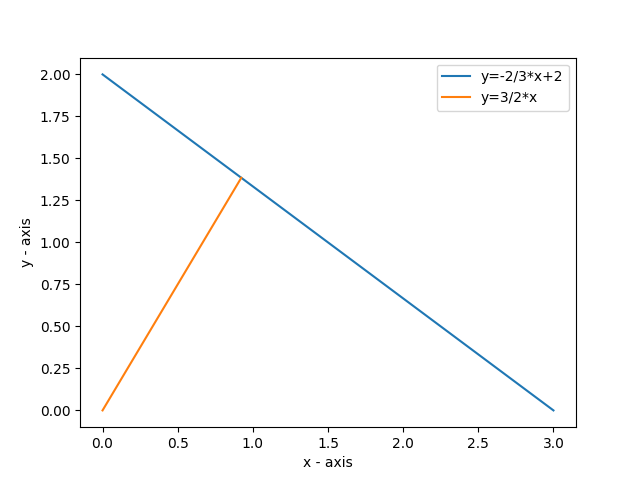
\includegraphics[width=\columnwidth]{Figure_1.png}
        
        \label{fig:fig1}
    \end{figure}
\end{frame}

\end{document}
